\documentclass[tikz]{standalone}
\usepackage{tikz}
\usetikzlibrary{positioning, graphs}
\usetikzlibrary{graphs.standard}
\begin{document}
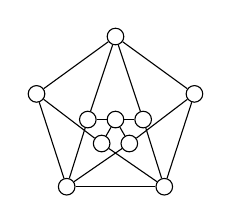
\begin{tikzpicture}
		[every node/.style={draw,circle,inner sep = 0em, minimum size = 0.6em}]
		\graph[clockwise, radius = 3em, empty nodes]{subgraph C_n[n = 5, name = A]};
		\graph[circular placement, phase = 180, radius = 1em, empty nodes]{a, b, c, d};
		
		\draw (0,0) node (P) {};
		
		\draw (A 1) -- (a);
		\draw (A 4) -- (a);
		\draw (P) -- (a);
		\draw (A 5) -- (b);
		\draw (A 3) -- (b);
		\draw (P) -- (b);
		\draw (A 2) -- (c);
		\draw (A 4) -- (c);
		\draw (P) -- (c);
		\draw (A 1) -- (d);
		\draw (A 3) -- (d);
		\draw (P) -- (d);
		
		%\foreach \i [evaluate={\j=int(mod(\i+1,3)+1); \k=int(mod(\i+2,3)+1);}] in {1, 2, 3}{
			%\draw (A \i) -- (B \j);
			%\draw (A \i) -- (B \k);
			%\draw (B \j) -- (C \i);
			%\draw (B \i) -- (C \k);
			%\draw (C \i) -- (a);
		%}
\end{tikzpicture}
\end{document}